%! suppress = MissingLabel
\documentclass[12pt,letterpaper,oneside,reqno]{amsart}
\usepackage{amsfonts}
\usepackage{amsmath}
\usepackage{amssymb}
\usepackage{amsthm}
\usepackage{float}
\usepackage{mathrsfs}
\usepackage[font=small,labelfont=bf]{caption}
\usepackage[left=1in,right=1in,bottom=1in,top=1in]{geometry}
\usepackage[pdfpagelabels,hyperindex,colorlinks=true,linkcolor=blue,urlcolor=magenta,citecolor=green]{hyperref}
\usepackage{graphicx}
\linespread{1.7}
\emergencystretch=1em
\usepackage{array}
\usepackage{etoolbox}
\apptocmd{\sloppy}{\hbadness 10000\relax}{}{}
\raggedbottom

\newcommand \anglePower [2]{\langle #1 \rangle \sp{#2}}
\newcommand \bernoulli [2][B] {{#1}\sb{#2}}
\newcommand \curvePower [2]{\{#1\}\sp{#2}}
\newcommand \coeffA [3][A] {{\mathbf{#1}} \sb{#2,#3}}
\newcommand \polynomialP [4][P]{{#1}(#2,#3,#4)}
\newcommand \polynomialQ [4][Q]{{#1}(#2,#3,#4)}

\newtheorem{theorem}{Theorem}[section]
\newtheorem{corollary}[theorem]{Corollary}
\newtheorem{lemma}[theorem]{Lemma}
\newtheorem{example}[theorem]{Example}
\newtheorem{conjecture}[theorem]{Conjecture}
\newtheorem{definition}[theorem]{Definition}

\title[Plots of Closed Forms]
{Plots of Closed Forms}
\author[Petro Kolosov]{Petro Kolosov}
\hypersetup{
    pdftitle={Plots of Closed Forms},
    pdfsubject={
        Polynomials,
        Finite differences,
        Interpolation,
        Approximation,
        Polynomial identities,
        Power sums,
        Binomial theorem,
        Power function,
        Binomial coefficients,
        Bernoulli numbers,
        Pascal's triangle,
        Faulhaber's formula
    },
    pdfauthor={Petro Kolosov},
    pdfkeywords={
        Polynomials,
        Finite differences,
        Interpolation,
        Approximation,
        Polynomial identities,
        Power sums,
        Binomial theorem,
        Power function,
        Binomial coefficients,
        Bernoulli numbers,
        Pascal's triangle,
        Faulhaber's formula
    }
}
\begin{document}

    \begin{abstract}
        Let $P(m, X, N)$ and $Q(m, X, N)$ be $m$-degree polynomials in $X\in\mathbb{R}$
having fixed non-negative integer values for $m$ and $N$.
In this manuscript an efficient method of spline approximation for power function is shown and discussed.
Approximation technique is based on the fact that both $P(m, X, N)$ and $Q(m, X, N)$
approximate the polynomial $X^{2m+1}$ in for $a$ in some neighborhood of fixed $N$.

    \end{abstract}

    \maketitle

    \tableofcontents


    \section{Introduction}\label{sec:introduction}
    Definitions
    \begin{align*}
        \polynomialP{m}{X}{N} &= \sum_{r=0}^{m} \sum_{k=1}^{N} \coeffA{m}{r} k^r (X-k)^r \\
        \polynomialP{m}{X}{N} &= \sum_{r=0}^{m} (-1)^{m-r} U(m, N, r) \cdot X^{r} \\
        \polynomialQ{m}{X}{N} &= \sum_{r=0}^{m} \sum_{k=0}^{N-1} \coeffA{m}{r} k^r (X-k)^r \\
        \polynomialQ{m}{X}{N} &= \sum_{r=0}^{m} (-1)^{m-r} V(m, N, r) \cdot X^{r} \\
        U(m, l, t) &= (-1)^m \sum_{k=1}^{l} \sum_{j=t}^{m} \binom{j}{t} \coeffA{m}{j} k^{2j-t} (-1)^j \\
        V(m, l, t) &= (-1)^m \sum_{k=0}^{l-1}  \sum_{j=t}^{m} \binom{j}{t} \coeffA{m}{j} k^{2j-t} (-1)^j
    \end{align*}

    Polynomial identities found, these polynomial identities allow us to assume that $N-1, N, N+1$ interval
    has quite precise convergence.
    \begin{align*}
        \polynomialP{m}{N}{N} &= N^{2m+1} \\
        \polynomialQ{m}{N}{N} &= N^{2m+1} \\
        \polynomialP{m}{N+1}{N} &= (N+1)^{2m+1} - 1 \quad \quad (verified) \\
        \polynomialQ{m}{N-1}{N} &= (N-1)^{2m+1} + 1 \quad \quad (verified)
    \end{align*}

    The function $U(m, N, r)$ rises as $O(N^{2m+1-r})$ having fixed values for $m$ and $r$
    \begin{align*}
        U(m, N, r) &= O(N^{2m+1-r}) \\
        U(3, N, 1) &= 70 N^6+210 N^5+175 N^4-42 N^2-7 N
    \end{align*}

    The function $V(m, N, r)$ rises as $O(N^{2m+1-r})$ having fixed values for $m$ and $r$
    \begin{align*}
        V(m, N, r) &= O(N^{2m+1-r}) \\
        V(3, N, 2) &= -14 N + 140 N^3 - 210 N^4 + 84 N^5
    \end{align*}

    Error of approximation, fixed $m$ and $N$
    \begin{align*}
        E &= (X+1)^{2m+1} - \polynomialP{m}{X}{N} \\
        E &= \sum_{k=0}^{N} \binom{N}{k} X^k - \polynomialP{m}{X}{N}
    \end{align*}

    About interval of convergence, we say that having fixed points $m$ and $N$,
    the polynomial $\polynomialP{m}{X}{N}$ approximates odd power function $X^{2m+1}$ in some interval
    of convergence $a_1 \leq N \leq b_1$.
    For example,
    \begin{align*}
        \polynomialP{1}{X}{6} = 126X - 540
    \end{align*}
    so that it approximates odd power function $X^3$ in some neighborhood of point $X=6$, more precisely
    $5.5 \leq X \leq 7.9$ with the maximal percentage error $8\%$.

    Having $N=10$ the convergence interval with cubes in neighborhood of $X=10$ is: $8.9 \leq X \leq 13$
    with maximal percentage error $E \leq 10\%$.

    Having $N=70$ the convergence interval with cubes in neighborhood of $X=70$ is: $60.1 \leq X \leq 87.6$
    with maximal percentage error $E \leq 10\%$.

    Having $N=150$ the convergence interval with cubes in neighborhood of $X=150$ is: $128.4 \leq X \leq 187.1$
    with maximal percentage error $E \leq 10\%$.
    Within interval $142.5 \leq X \leq 159.9$ the maximal percentage error $E < 1\%$.

    Which implies that convergence interval rises as $N$ rise.

    Which makes the method quite fit for spline approximation.

    % P1
    \clearpage

    \subsection{Polynomials P(1,X,N)}
    \begin{align*}
    \polynomialP{1}{X}{0} &= 0 \\
    \polynomialP{1}{X}{1} &= 6X - 5 \\
    \polynomialP{1}{X}{2} &= 18X - 28 \\
    \polynomialP{1}{X}{3} &= 36X - 81 \\
    \polynomialP{1}{X}{4} &= 60X - 176 \\
    \polynomialP{1}{X}{5} &= 90X - 325 \\
    \polynomialP{1}{X}{6} &= 126X - 540 \\
    \polynomialP{1}{X}{7} &= 168X - 833 \\
    \polynomialP{1}{X}{8} &= 216X - 1216 \\
    \polynomialP{1}{X}{9} &= 270X - 1701 \\
    \polynomialP{1}{X}{10} &= 330X - 2300 \\
    \polynomialP{1}{X}{11} &= 396X - 3025 \\
    \polynomialP{1}{X}{12} &= 468X - 3888 \\
    \polynomialP{1}{X}{13} &= 546X - 4901 \\
    \polynomialP{1}{X}{14} &= 630X - 6076 \\
    \polynomialP{1}{X}{15} &= 720X - 7425 \\
    \polynomialP{1}{X}{16} &= 816X - 8960 \\
    \polynomialP{1}{X}{17} &= 918X - 10693 \\
    \polynomialP{1}{X}{18} &= 1026X - 12636 \\
    \polynomialP{1}{X}{19} &= 1140X - 14801 \\
    \polynomialP{1}{X}{20} &= 1260X - 17200
\end{align*}
\begin{figure}[H]
    \centering
    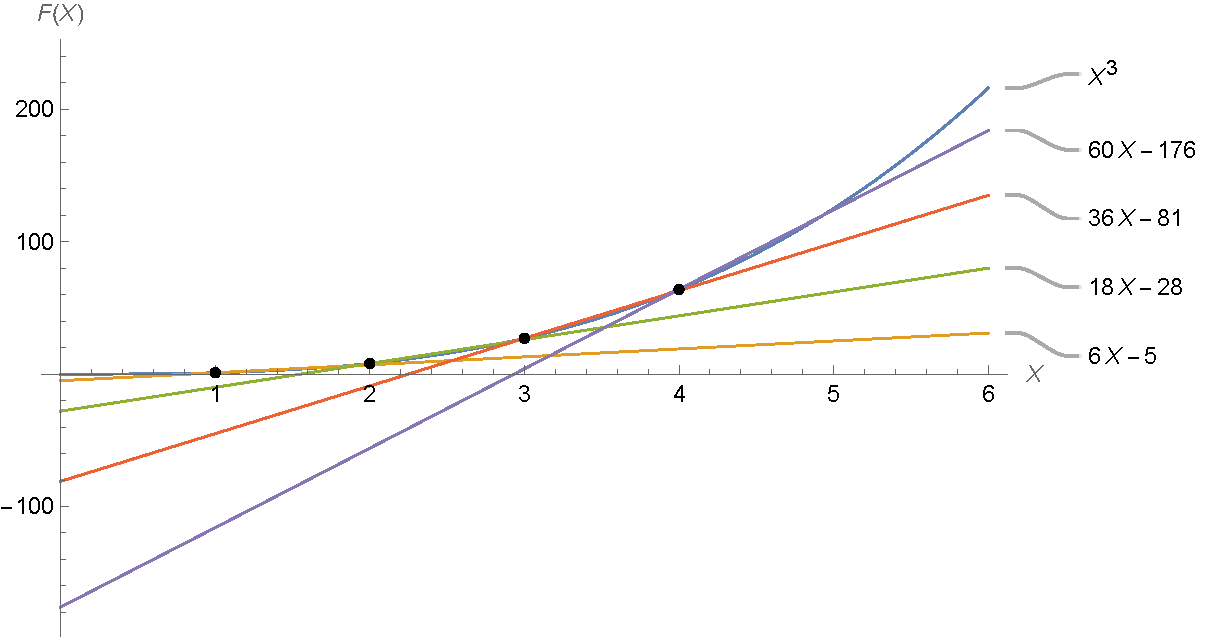
\includegraphics[width=1\textwidth]{sections/images/01_plots_cubes_with_p1}
    ~\caption{Polynomials $P(1, X, N)$ for N=1..4}\label{fig:figure}
\end{figure}


    \subsection{Polynomial P(1,X,N) Table of values for N = 6}
    \begin{table}[h!]
    \centering
    \caption{Comparison of $X^3$, $\polynomialP{1}{X}{6} =126X-540$, Absolute, Relative, and Percentage Error}
    \begin{tabular}{|c|c|c|c|c|c|}
        \hline
        \textbf{X} & \textbf{$X^3$} & \textbf{$126X-540$} & \textbf{ABS} & \textbf{Relative} & \textbf{\% Error} \\ \hline
        5.3        & 148.877        & 127.8               & 21.077       & 0.141573          & 14.1573           \\ \hline
        5.4        & 157.464        & 140.4               & 17.064       & 0.108368          & 10.8368           \\ \hline
        5.5        & 166.375        & 153.0               & 13.375       & 0.0803907         & 8.03907           \\ \hline
        5.6        & 175.616        & 165.6               & 10.016       & 0.0570335         & 5.70335           \\ \hline
        5.7        & 185.193        & 178.2               & 6.993        & 0.0377606         & 3.77606           \\ \hline
        5.8        & 195.112        & 190.8               & 4.312        & 0.0221001         & 2.21001           \\ \hline
        5.9        & 205.379        & 203.4               & 1.979        & 0.00963584        & 0.963584          \\ \hline
        6.0        & 216.0          & 216.0               & 0.0          & 0.0               & 0.0               \\ \hline
        6.1        & 226.981        & 228.6               & 1.619        & 0.00713276        & 0.713276          \\ \hline
        6.2        & 238.328        & 241.2               & 2.872        & 0.0120506         & 1.20506           \\ \hline
        6.3        & 250.047        & 253.8               & 3.753        & 0.0150092         & 1.50092           \\ \hline
        6.4        & 262.144        & 266.4               & 4.256        & 0.0162354         & 1.62354           \\ \hline
        6.5        & 274.625        & 279.0               & 4.375        & 0.0159308         & 1.59308           \\ \hline
        6.6        & 287.496        & 291.6               & 4.104        & 0.014275          & 1.4275            \\ \hline
        6.7        & 300.763        & 304.2               & 3.437        & 0.0114276         & 1.14276           \\ \hline
        6.8        & 314.432        & 316.8               & 2.368        & 0.00753104        & 0.753104          \\ \hline
        6.9        & 328.509        & 329.4               & 0.891        & 0.00271225        & 0.271225          \\ \hline
        7.0        & 343.0          & 342.0               & 1.0          & 0.00291545        & 0.291545          \\ \hline
        7.1        & 357.911        & 354.6               & 3.311        & 0.0092509         & 0.92509           \\ \hline
        7.2        & 373.248        & 367.2               & 6.048        & 0.0162037         & 1.62037           \\ \hline
        7.3        & 389.017        & 379.8               & 9.217        & 0.0236931         & 2.36931           \\ \hline
        7.4        & 405.224        & 392.4               & 12.824       & 0.0316467         & 3.16467           \\ \hline
        7.5        & 421.875        & 405.0               & 16.875       & 0.04              & 4.0               \\ \hline
        7.6        & 438.976        & 417.6               & 21.376       & 0.0486951         & 4.86951           \\ \hline
        7.7        & 456.533        & 430.2               & 26.333       & 0.0576804         & 5.76804           \\ \hline
        7.8        & 474.552        & 442.8               & 31.752       & 0.0669094         & 6.69094           \\ \hline
        7.9        & 493.039        & 455.4               & 37.639       & 0.0763408         & 7.63408           \\ \hline
        8.0        & 512.0          & 468.0               & 44.0         & 0.0859375         & 8.59375           \\ \hline
        8.1        & 531.441        & 480.6               & 50.841       & 0.0956663         & 9.56663           \\ \hline
        8.2        & 551.368        & 493.2               & 58.168       & 0.105498          & 10.5498           \\ \hline
    \end{tabular}\label{tab:table}
\end{table}


    \subsection{Polynomial P(1,X,6) plot with cubes}
    \begin{figure}[H]
    \centering
    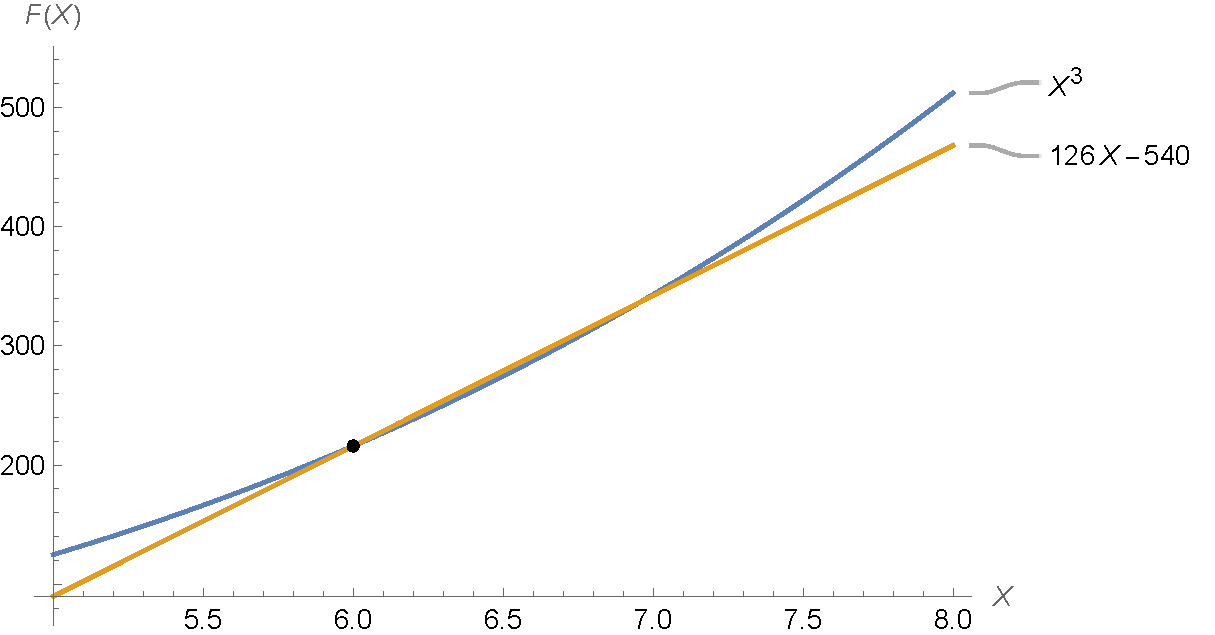
\includegraphics[width=1\textwidth]{sections/images/01_plots_polynomial_p1_n6_with_cubes}
    ~\caption{Polynomial plot P(1, X, 6) with cubes $X^3$.
    Points of intersection $X=6$, $X=6.94987$.}\label{fig:figure7}
\end{figure}


    % Q1

    \subsection{Polynomials Q(1,X,N)}
    \begin{align*}
    \polynomialQ{1}{X}{0} &= 0 \\
    \polynomialQ{1}{X}{1} &= 1 \\
    \polynomialQ{1}{X}{2} &= 6X - 4 \\
    \polynomialQ{1}{X}{3} &= 18X - 27 \\
    \polynomialQ{1}{X}{4} &= 36X - 80 \\
    \polynomialQ{1}{X}{5} &= 60X - 175 \\
    \polynomialQ{1}{X}{6} &= 90X - 324 \\
    \polynomialQ{1}{X}{7} &= 126X - 539 \\
    \polynomialQ{1}{X}{8} &= 168X - 832 \\
    \polynomialQ{1}{X}{9} &= 216X - 1215 \\
    \polynomialQ{1}{X}{10} &= 270X - 1700 \\
    \polynomialQ{1}{X}{11} &= 330X - 2299 \\
    \polynomialQ{1}{X}{12} &= 396X - 3024 \\
    \polynomialQ{1}{X}{13} &= 468X - 3887 \\
    \polynomialQ{1}{X}{14} &= 546X - 4900 \\
    \polynomialQ{1}{X}{15} &= 630X - 6075 \\
    \polynomialQ{1}{X}{16} &= 720X - 7424 \\
    \polynomialQ{1}{X}{17} &= 816X - 8959 \\
    \polynomialQ{1}{X}{18} &= 918X - 10692 \\
    \polynomialQ{1}{X}{19} &= 1026X - 12635 \\
    \polynomialQ{1}{X}{20} &= 1140X - 14800
\end{align*}
\begin{figure}[H]
    \centering
    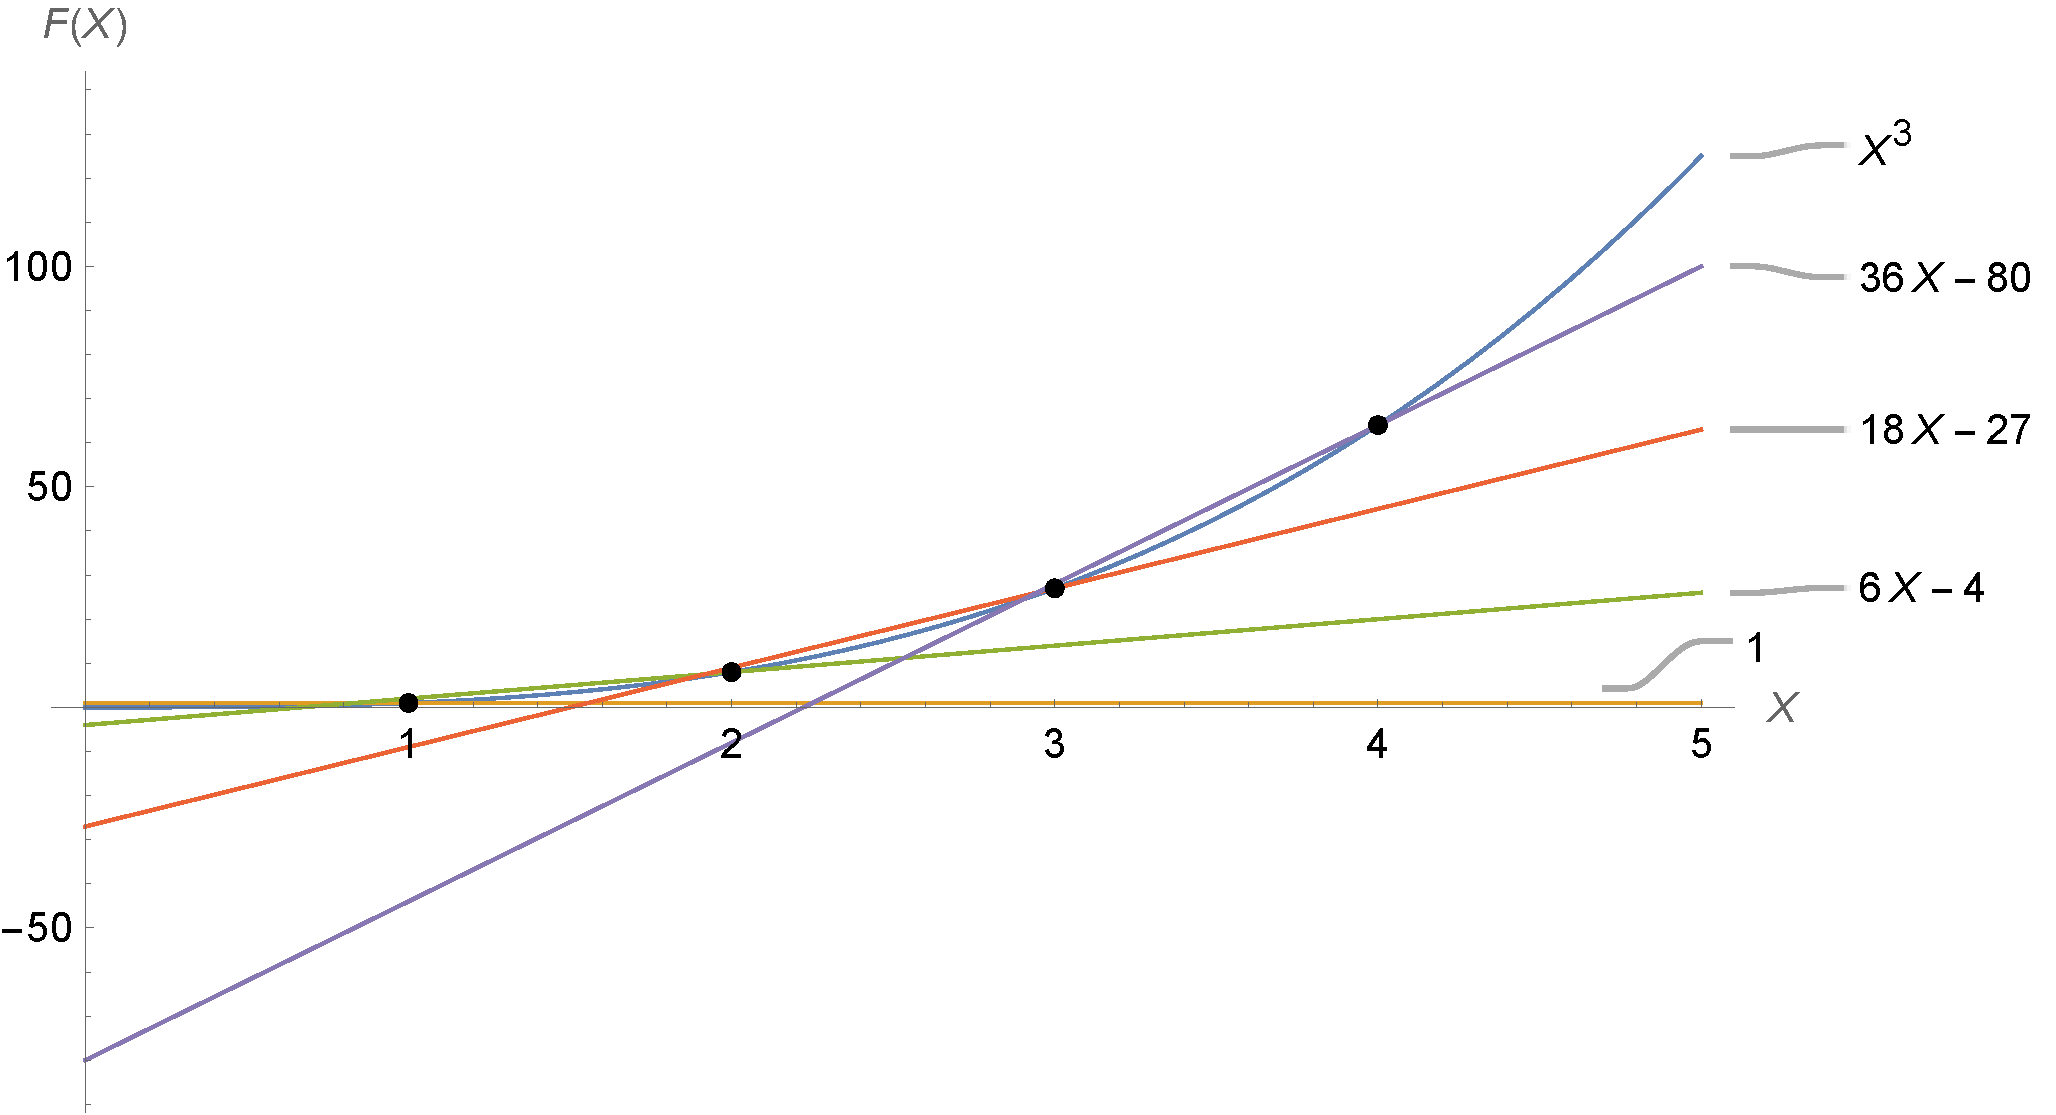
\includegraphics[width=1\textwidth]{sections/images/02_plots_cubes_with_q1}
    ~\caption{Polynomials Q(1, n, k)}\label{fig:figure2}
\end{figure}



    \subsection{Polynomial Q(1,X,N) Table of values for N = 6}
    \begin{table}[h!]
    \centering
    \caption{Comparison of $X^3$, $\polynomialQ{1}{X}{6} = 90X-324$, Absolute, Relative, and Percentage Error}
    \begin{tabular}{|c|c|c|c|c|c|}
        \hline
        \textbf{X} & \textbf{$X^3$} & \textbf{$90X-324$} & \textbf{ABS} & \textbf{Relative} & \textbf{\% Error} \\ \hline
        4.5        & 91.125         & 81.0               & 10.125       & 0.111111          & 11.1111           \\ \hline
        4.6        & 97.336         & 90.0               & 7.336        & 0.0753678         & 7.53678           \\ \hline
        4.7        & 103.823        & 99.0               & 4.823        & 0.0464541         & 4.64541           \\ \hline
        4.8        & 110.592        & 108.0              & 2.592        & 0.0234375         & 2.34375           \\ \hline
        4.9        & 117.649        & 117.0              & 0.649        & 0.00551641        & 0.551641          \\ \hline
        5.0        & 125.0          & 126.0              & 1.0          & 0.008             & 0.8               \\ \hline
        5.1        & 132.651        & 135.0              & 2.349        & 0.0177081         & 1.77081           \\ \hline
        5.2        & 140.608        & 144.0              & 3.392        & 0.0241238         & 2.41238           \\ \hline
        5.3        & 148.877        & 153.0              & 4.123        & 0.027694          & 2.7694            \\ \hline
        5.4        & 157.464        & 162.0              & 4.536        & 0.0288066         & 2.88066           \\ \hline
        5.5        & 166.375        & 171.0              & 4.625        & 0.0277986         & 2.77986           \\ \hline
        5.6        & 175.616        & 180.0              & 4.384        & 0.0249636         & 2.49636           \\ \hline
        5.7        & 185.193        & 189.0              & 3.807        & 0.0205569         & 2.05569           \\ \hline
        5.8        & 195.112        & 198.0              & 2.888        & 0.0148018         & 1.48018           \\ \hline
        5.9        & 205.379        & 207.0              & 1.621        & 0.00789273        & 0.789273          \\ \hline
        6.0        & 216.0          & 216.0              & 0.0          & 0.0               & 0.0               \\ \hline
        6.1        & 226.981        & 225.0              & 1.981        & 0.0087276         & 0.87276           \\ \hline
        6.2        & 238.328        & 234.0              & 4.328        & 0.0181598         & 1.81598           \\ \hline
        6.3        & 250.047        & 243.0              & 7.047        & 0.0281827         & 2.81827           \\ \hline
        6.4        & 262.144        & 252.0              & 10.144       & 0.0386963         & 3.86963           \\ \hline
        6.5        & 274.625        & 261.0              & 13.625       & 0.0496131         & 4.96131           \\ \hline
        6.6        & 287.496        & 270.0              & 17.496       & 0.0608565         & 6.08565           \\ \hline
        6.7        & 300.763        & 279.0              & 21.763       & 0.0723593         & 7.23593           \\ \hline
        6.8        & 314.432        & 288.0              & 26.432       & 0.0840627         & 8.40627           \\ \hline
        6.9        & 328.509        & 297.0              & 31.509       & 0.0959152         & 9.59152           \\ \hline
        7.0        & 343.0          & 306.0              & 37.0         & 0.107872          & 10.7872           \\ \hline
    \end{tabular}\label{tab:table4}
\end{table}


    \subsection{Polynomial Q(1,X,6) plot with cubes}
    \begin{figure}[H]
    \centering
    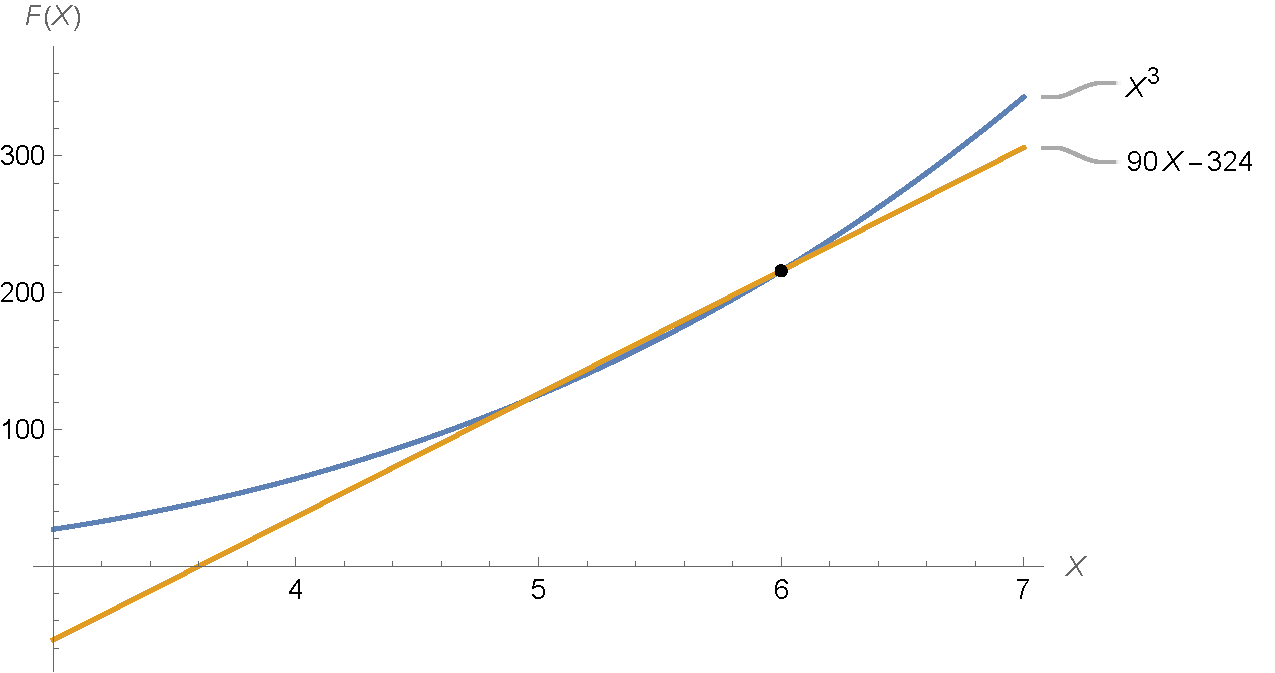
\includegraphics[width=1\textwidth]{sections/images/02_plots_polynomial_q1_n6_with_cubes}
    ~\caption{Polynomial plot Q(1, X, 6) with cubes}\label{fig:figure8}
\end{figure}


    % P2

    \subsection{Polynomials P(2,X,N)}
    \begin{align*}
    \polynomialP{2}{X}{0} &= 0 \\
    \polynomialP{2}{X}{1} &= 30X^2 - 60X + 31 \\
    \polynomialP{2}{X}{2} &= 150X^2 - 540X + 512 \\
    \polynomialP{2}{X}{3} &= 420X^2 - 2160X + 2943 \\
    \polynomialP{2}{X}{4} &= 900X^2 - 6000X + 10624 \\
    \polynomialP{2}{X}{5} &= 1650X^2 - 13500X + 29375 \\
    \polynomialP{2}{X}{6} &= 2730X^2 - 26460X + 68256 \\
    \polynomialP{2}{X}{7} &= 4200X^2 - 47040X + 140287 \\
    \polynomialP{2}{X}{8} &= 6120X^2 - 77760X + 263168 \\
    \polynomialP{2}{X}{9} &= 8550X^2 - 121500X + 459999 \\
    \polynomialP{2}{X}{10} &= 11550X^2 - 181500X + 760000 \\
    \polynomialP{2}{X}{11} &= 15180X^2 - 261360X + 1199231 \\
    \polynomialP{2}{X}{12} &= 19500X^2 - 365040X + 1821312 \\
    \polynomialP{2}{X}{13} &= 24570X^2 - 496860X + 2678143 \\
    \polynomialP{2}{X}{14} &= 30450X^2 - 661500X + 3830624 \\
    \polynomialP{2}{X}{15} &= 37200X^2 - 864000X + 5349375 \\
    \polynomialP{2}{X}{16} &= 44880X^2 - 1109760X + 7315456 \\
    \polynomialP{2}{X}{17} &= 53550X^2 - 1404540X + 9821087 \\
    \polynomialP{2}{X}{18} &= 63270X^2 - 1754460X + 12970368 \\
    \polynomialP{2}{X}{19} &= 74100X^2 - 2166000X + 16879999 \\
    \polynomialP{2}{X}{20} &= 86100X^2 - 2646000X + 21680000
\end{align*}
\begin{figure}[H]
    \centering
    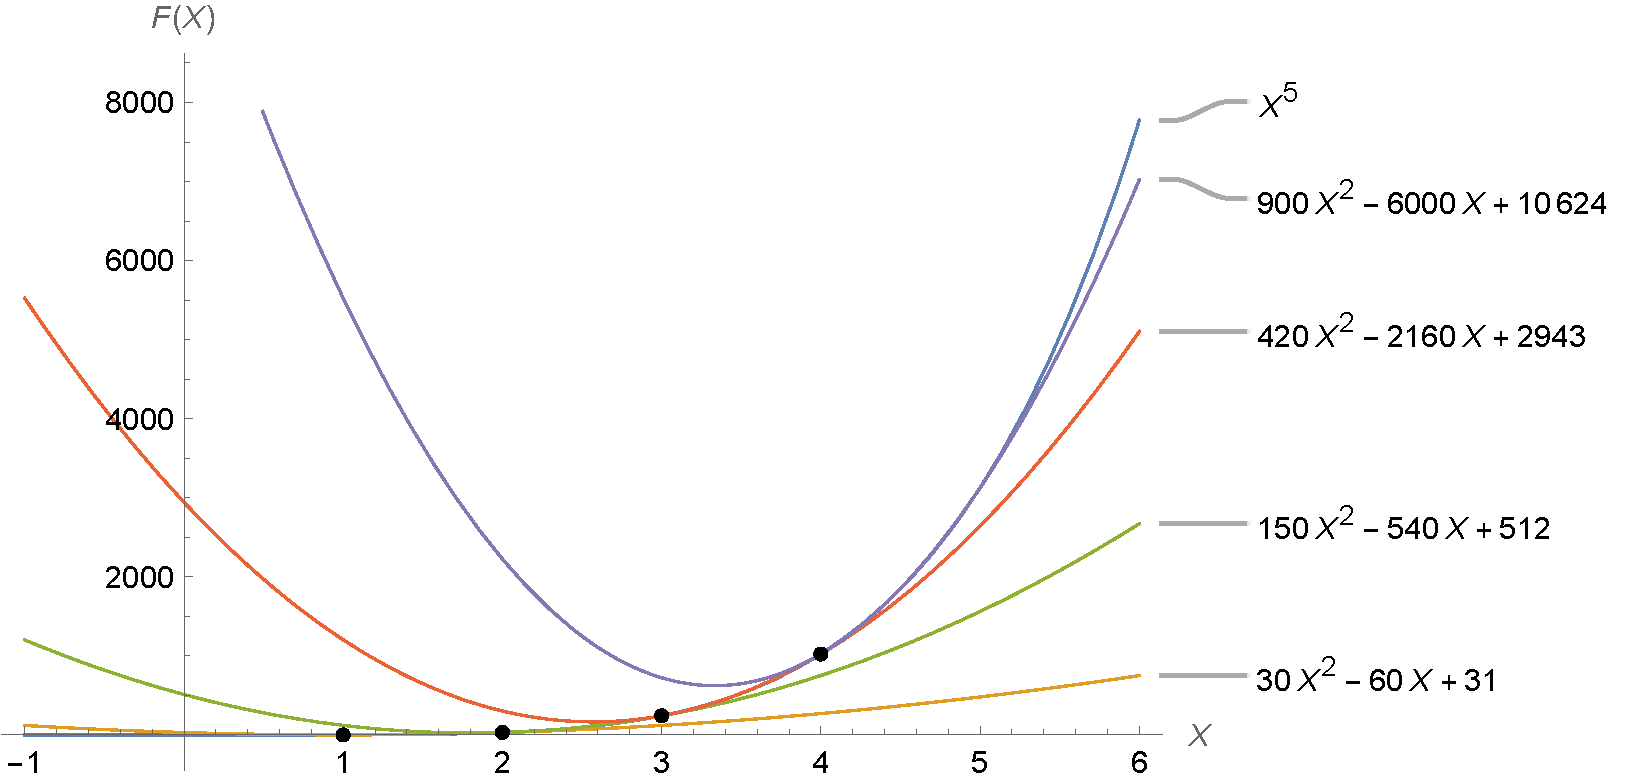
\includegraphics[width=1\textwidth]{sections/images/03_plots_fifth_with_p2}
    ~\caption{Polynomials P(2, n, k)}\label{fig:figure3}
\end{figure}


    \subsection{Polynomial P(2,X,N) Table of values for N = 4}
    \begin{table}[h!]
    \centering
    \caption{Comparison of $X^5$, $\polynomialP{2}{X}{4} = 900X^2 - 6000X + 10624$, Absolute, Relative, and Percentage Error}
    \begin{tabular}{|c|c|c|c|c|c|}
        \hline
        \textbf{X} & \textbf{$X^5$} & \textbf{$900X^2 - 6000X + 10624$} & \textbf{ABS} & \textbf{Relative} & \textbf{\% Error} \\ \hline
        3.6        & 604.662        & 688.0                             & 83.3382      & 0.137826          & 13.7826           \\ \hline
        3.7        & 693.44         & 745.0                             & 51.5604      & 0.0743546         & 7.43546           \\ \hline
        3.8        & 792.352        & 820.0                             & 27.6483      & 0.034894          & 3.4894            \\ \hline
        3.9        & 902.242        & 913.0                             & 10.758       & 0.0119236         & 1.19236           \\ \hline
        4.0        & 1024.0         & 1024.0                            & 0.0          & 0.0               & 0.0               \\ \hline
        4.1        & 1158.56        & 1153.0                            & 5.56201      & 0.00480079        & 0.480079          \\ \hline
        4.2        & 1306.91        & 1300.0                            & 6.91232      & 0.00528905        & 0.528905          \\ \hline
        4.3        & 1470.08        & 1465.0                            & 5.08443      & 0.0034586         & 0.34586           \\ \hline
        4.4        & 1649.16        & 1648.0                            & 1.16224      & 0.000704746       & 0.0704746         \\ \hline
        4.5        & 1845.28        & 1849.0                            & 3.71875      & 0.00201528        & 0.201528          \\ \hline
        4.6        & 2059.63        & 2068.0                            & 8.37024      & 0.00406395        & 0.406395          \\ \hline
        4.7        & 2293.45        & 2305.0                            & 11.5499      & 0.00503605        & 0.503605          \\ \hline
        4.8        & 2548.04        & 2560.0                            & 11.9603      & 0.00469393        & 0.469393          \\ \hline
        4.9        & 2824.75        & 2833.0                            & 8.24751      & 0.00291973        & 0.291973          \\ \hline
        5.0        & 3125.0         & 3124.0                            & 1.0          & 0.00032           & 0.032             \\ \hline
        5.1        & 3450.25        & 3433.0                            & 17.2525      & 0.00500036        & 0.500036          \\ \hline
        5.2        & 3802.04        & 3760.0                            & 42.0403      & 0.0110573         & 1.10573           \\ \hline
        5.3        & 4181.95        & 4105.0                            & 76.9549      & 0.0184017         & 1.84017           \\ \hline
        5.4        & 4591.65        & 4468.0                            & 123.65       & 0.0269294         & 2.69294           \\ \hline
        5.5        & 5032.84        & 4849.0                            & 183.844      & 0.0365288         & 3.65288           \\ \hline
        5.6        & 5507.32        & 5248.0                            & 259.318      & 0.047086          & 4.7086            \\ \hline
        5.7        & 6016.92        & 5665.0                            & 351.921      & 0.0584885         & 5.84885           \\ \hline
        5.8        & 6563.57        & 6100.0                            & 463.568      & 0.0706274         & 7.06274           \\ \hline
        5.9        & 7149.24        & 6553.0                            & 596.243      & 0.0833995         & 8.33995           \\ \hline
        6.0        & 7776.0         & 7024.0                            & 752.0        & 0.0967078         & 9.67078           \\ \hline
        6.1        & 8445.96        & 7513.0                            & 932.963      & 0.110463          & 11.0463           \\ \hline
    \end{tabular}\label{tab:table2}
\end{table}


    \subsection{Polynomial P(2,X,4) plot with fifth}
    \begin{figure}[H]
    \centering
    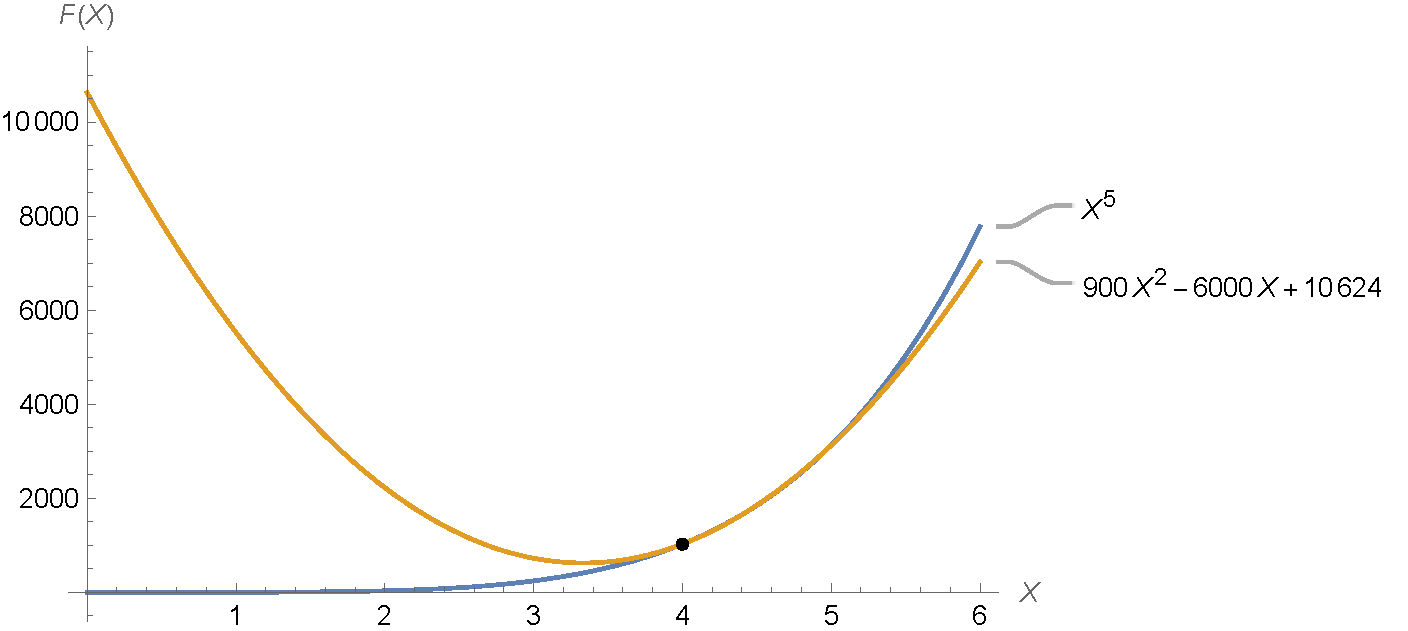
\includegraphics[width=1\textwidth]{sections/images/03_plots_polynomial_p2_n4_with_fifth}
    ~\caption{Polynomial plot $P(2, X, 4)$ with fifth power $X^5$.
    Points of intersection $X=4$, $X=4.42472$, $X=4.99181$.
    Interval of convergence: $3.9 \leq X \leq 5.3$.
    }\label{fig:figure9}
\end{figure}


    % Q2

    \subsection{Polynomials Q(2,X,N)}
    \begin{align*}
    \polynomialQ{2}{X}{0} &= 0 \\
    \polynomialQ{2}{X}{1} &= 1 \\
    \polynomialQ{2}{X}{2} &= 30X^2 - 60X + 32 \\
    \polynomialQ{2}{X}{3} &= 150X^2 - 540X + 513 \\
    \polynomialQ{2}{X}{4} &= 420X^2 - 2160X + 2944 \\
    \polynomialQ{2}{X}{5} &= 900X^2 - 6000X + 10625 \\
    \polynomialQ{2}{X}{6} &= 1650X^2 - 13500X + 29376 \\
    \polynomialQ{2}{X}{7} &= 2730X^2 - 26460X + 68257 \\
    \polynomialQ{2}{X}{8} &= 4200X^2 - 47040X + 140288 \\
    \polynomialQ{2}{X}{9} &= 6120X^2 - 77760X + 263169 \\
    \polynomialQ{2}{X}{10} &= 8550X^2 - 121500X + 460000 \\
    \polynomialQ{2}{X}{11} &= 11550X^2 - 181500X + 760001 \\
    \polynomialQ{2}{X}{12} &= 15180X^2 - 261360X + 1199232 \\
    \polynomialQ{2}{X}{13} &= 19500X^2 - 365040X + 1821313 \\
    \polynomialQ{2}{X}{14} &= 24570X^2 - 496860X + 2678144 \\
    \polynomialQ{2}{X}{15} &= 30450X^2 - 661500X + 3830625 \\
    \polynomialQ{2}{X}{16} &= 37200X^2 - 864000X + 5349376 \\
    \polynomialQ{2}{X}{17} &= 44880X^2 - 1109760X + 7315457 \\
    \polynomialQ{2}{X}{18} &= 53550X^2 - 1404540X + 9821088 \\
    \polynomialQ{2}{X}{19} &= 63270X^2 - 1754460X + 12970369 \\
    \polynomialQ{2}{X}{20} &= 74100X^2 - 2166000X + 16880000
\end{align*}
\begin{figure}[H]
    \centering
    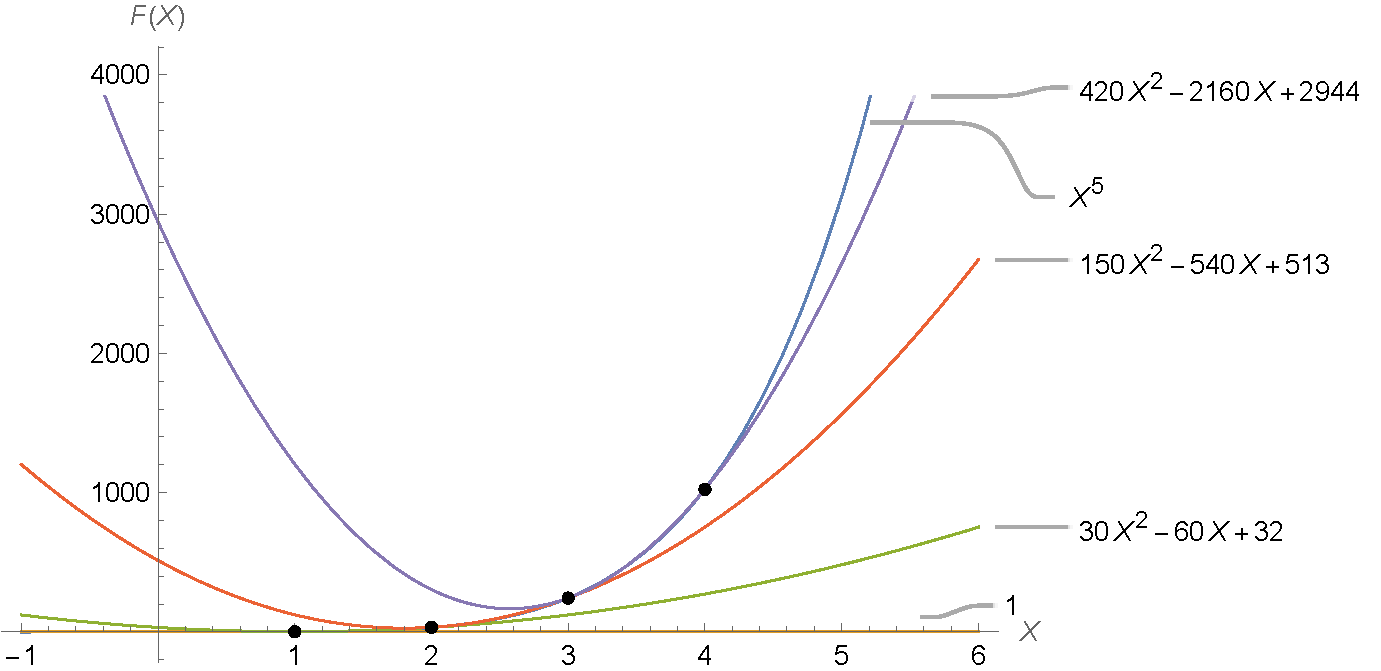
\includegraphics[width=1\textwidth]{sections/images/04_plots_fifth_with_q2}
    ~\caption{Polynomials Q(2, n, k)}\label{fig:figure4}
\end{figure}


    \subsection{Polynomial Q(2,X,N) Table of values for N = 4}
    \begin{table}[h!]
    \centering
    \caption{Comparison of $X^5$, $\polynomialQ{2}{X}{4} = 420X^2 - 2160X + 2944$, Absolute, Relative, and Percentage Error}
    \begin{tabular}{|c|c|c|c|c|c|}
        \hline
        \textbf{X} & \textbf{$X^5$} & \textbf{$420X^2-2160X+2944$} & \textbf{ABS} & \textbf{Relative} & \textbf{\% Error} \\ \hline
        2.7        & 143.489        & 173.8                        & 30.3109      & 0.211242          & 21.1242           \\ \hline
        2.8        & 172.104        & 188.8                        & 16.6963      & 0.0970131         & 9.70131           \\ \hline
        2.9        & 205.111        & 212.2                        & 7.08851      & 0.0345593         & 3.45593           \\ \hline
        3.0        & 243.0          & 244.0                        & 1.0          & 0.00411523        & 0.411523          \\ \hline
        3.1        & 286.292        & 284.2                        & 2.09151      & 0.00730553        & 0.730553          \\ \hline
        3.2        & 335.544        & 332.8                        & 2.74432      & 0.00817871        & 0.817871          \\ \hline
        3.3        & 391.354        & 389.8                        & 1.55393      & 0.00397065        & 0.397065          \\ \hline
        3.4        & 454.354        & 455.2                        & 0.84576      & 0.00186146        & 0.186146          \\ \hline
        3.5        & 525.219        & 529.0                        & 3.78125      & 0.00719938        & 0.719938          \\ \hline
        3.6        & 604.662        & 611.2                        & 6.53824      & 0.0108131         & 1.08131           \\ \hline
        3.7        & 693.44         & 701.8                        & 8.36043      & 0.0120565         & 1.20565           \\ \hline
        3.8        & 792.352        & 800.8                        & 8.44832      & 0.0106623         & 1.06623           \\ \hline
        3.9        & 902.242        & 908.2                        & 5.95801      & 0.00660356        & 0.660356          \\ \hline
        4.0        & 1024.0         & 1024.0                       & 0.0          & 0.0               & 0.0               \\ \hline
        4.1        & 1158.56        & 1148.2                       & 10.362       & 0.00894385        & 0.894385          \\ \hline
        4.2        & 1306.91        & 1280.8                       & 26.1123      & 0.0199802         & 1.99802           \\ \hline
        4.3        & 1470.08        & 1421.8                       & 48.2844      & 0.0328447         & 3.28447           \\ \hline
        4.4        & 1649.16        & 1571.2                       & 77.9622      & 0.0472738         & 4.72738           \\ \hline
        4.5        & 1845.28        & 1729.0                       & 116.281      & 0.0630155         & 6.30155           \\ \hline
        4.6        & 2059.63        & 1895.2                       & 164.43       & 0.0798346         & 7.98346           \\ \hline
        4.7        & 2293.45        & 2069.8                       & 223.65       & 0.0975169         & 9.75169           \\ \hline
        4.8        & 2548.04        & 2252.8                       & 295.24       & 0.115869          & 11.5869           \\ \hline
    \end{tabular}\label{tab:table5}
\end{table}


    \subsection{Polynomial Q(2,X,4) plot with fifth}
    \begin{figure}[H]
    \centering
    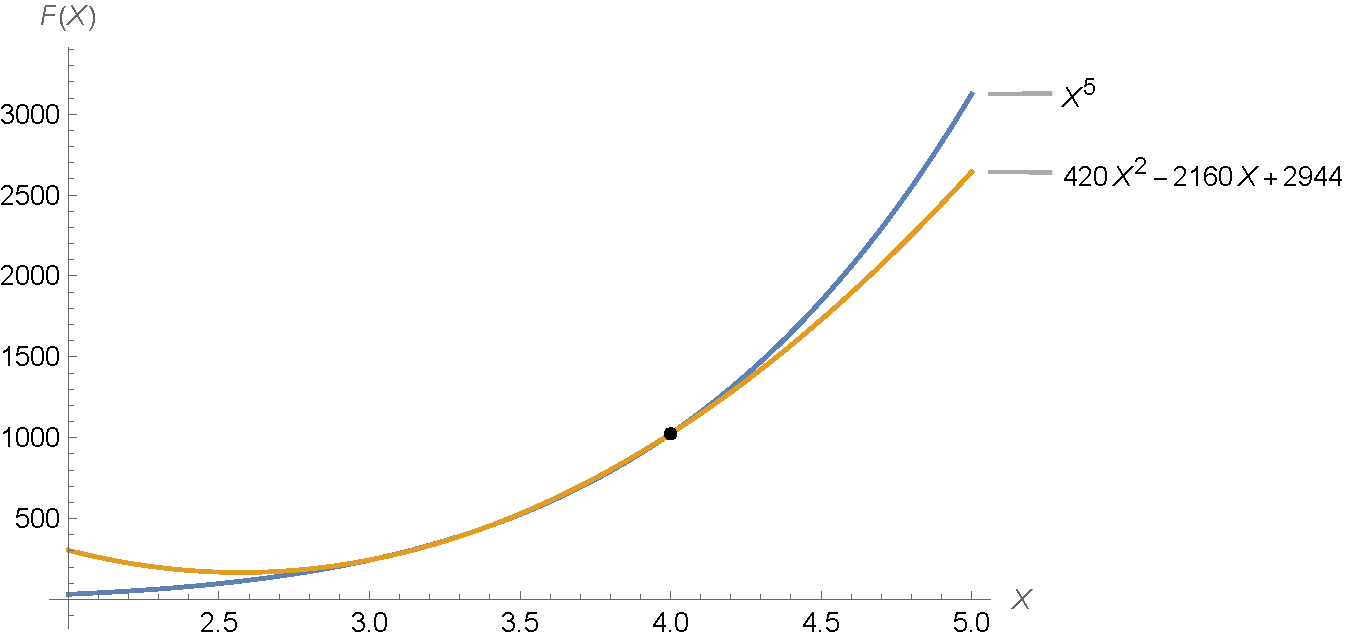
\includegraphics[width=1\textwidth]{sections/images/04_plots_polynomial_q2_n4_with_fifth}
    ~\caption{Polynomial plot Q(2, X, 4) with fifth}\label{fig:figure10}
\end{figure}


    % P3

    \subsection{Polynomials P(3,X,N)}
    \begin{align*}
    \polynomialP{3}{X}{0} &= 0 \\
    \polynomialP{3}{X}{1} &= 140X^3 - 420X^2 + 406X - 125 \\
    \polynomialP{3}{X}{2} &= 1260X^3 - 7140X^2 + 13818X - 9028 \\
    \polynomialP{3}{X}{3} &= 5040X^3 - 41160X^2 + 115836X - 110961 \\
    \polynomialP{3}{X}{4} &= 14000X^3 - 148680X^2 + 545860X - 684176 \\
    \polynomialP{3}{X}{5} &= 31500X^3 - 411180X^2 + 1858290X - 2871325 \\
    \polynomialP{3}{X}{6} &= 61740X^3 - 955500X^2 + 5124126X - 9402660 \\
    \polynomialP{3}{X}{7} &= 109760X^3 - 1963920X^2 + 12182968X - 25872833 \\
    \polynomialP{3}{X}{8} &= 181440X^3 - 3684240X^2 + 25945416X - 62572096 \\
    \polynomialP{3}{X}{9} &= 283500X^3 - 6439860X^2 + 50745870X - 136972701 \\
    \polynomialP{3}{X}{10} &= 423500X^3 - 10639860X^2 + 92745730X - 276971300 \\
    \polynomialP{3}{X}{11} &= 609840X^3 - 16789080X^2 + 160386996X - 524988145 \\
    \polynomialP{3}{X}{12} &= 851760X^3 - 25498200X^2 + 264896268X - 943023888 \\
    \polynomialP{3}{X}{13} &= 1159340X^3 - 37493820X^2 + 420839146X - 1618774781 \\
    \polynomialP{3}{X}{14} &= 1543500X^3 - 53628540X^2 + 646725030X - 2672907076 \\
    \polynomialP{3}{X}{15} &= 2016000X^3 - 74891040X^2 + 965662320X - 4267591425 \\
    \polynomialP{3}{X}{16} &= 2589440X^3 - 102416160X^2 + 1406064016X - 6616398080 \\
    \polynomialP{3}{X}{17} &= 3277260X^3 - 137494980X^2 + 2002403718X - 9995653693 \\
    \polynomialP{3}{X}{18} &= 4093740X^3 - 181584900X^2 + 2796022026X - 14757360516 \\
    \polynomialP{3}{X}{19} &= 5054000X^3 - 236319720X^2 + 3835983340X - 21343778801 \\
    \polynomialP{3}{X}{20} &= 6174000X^3 - 303519720X^2 + 5179983060X - 30303773200
\end{align*}
\begin{figure}[H]
    \centering
    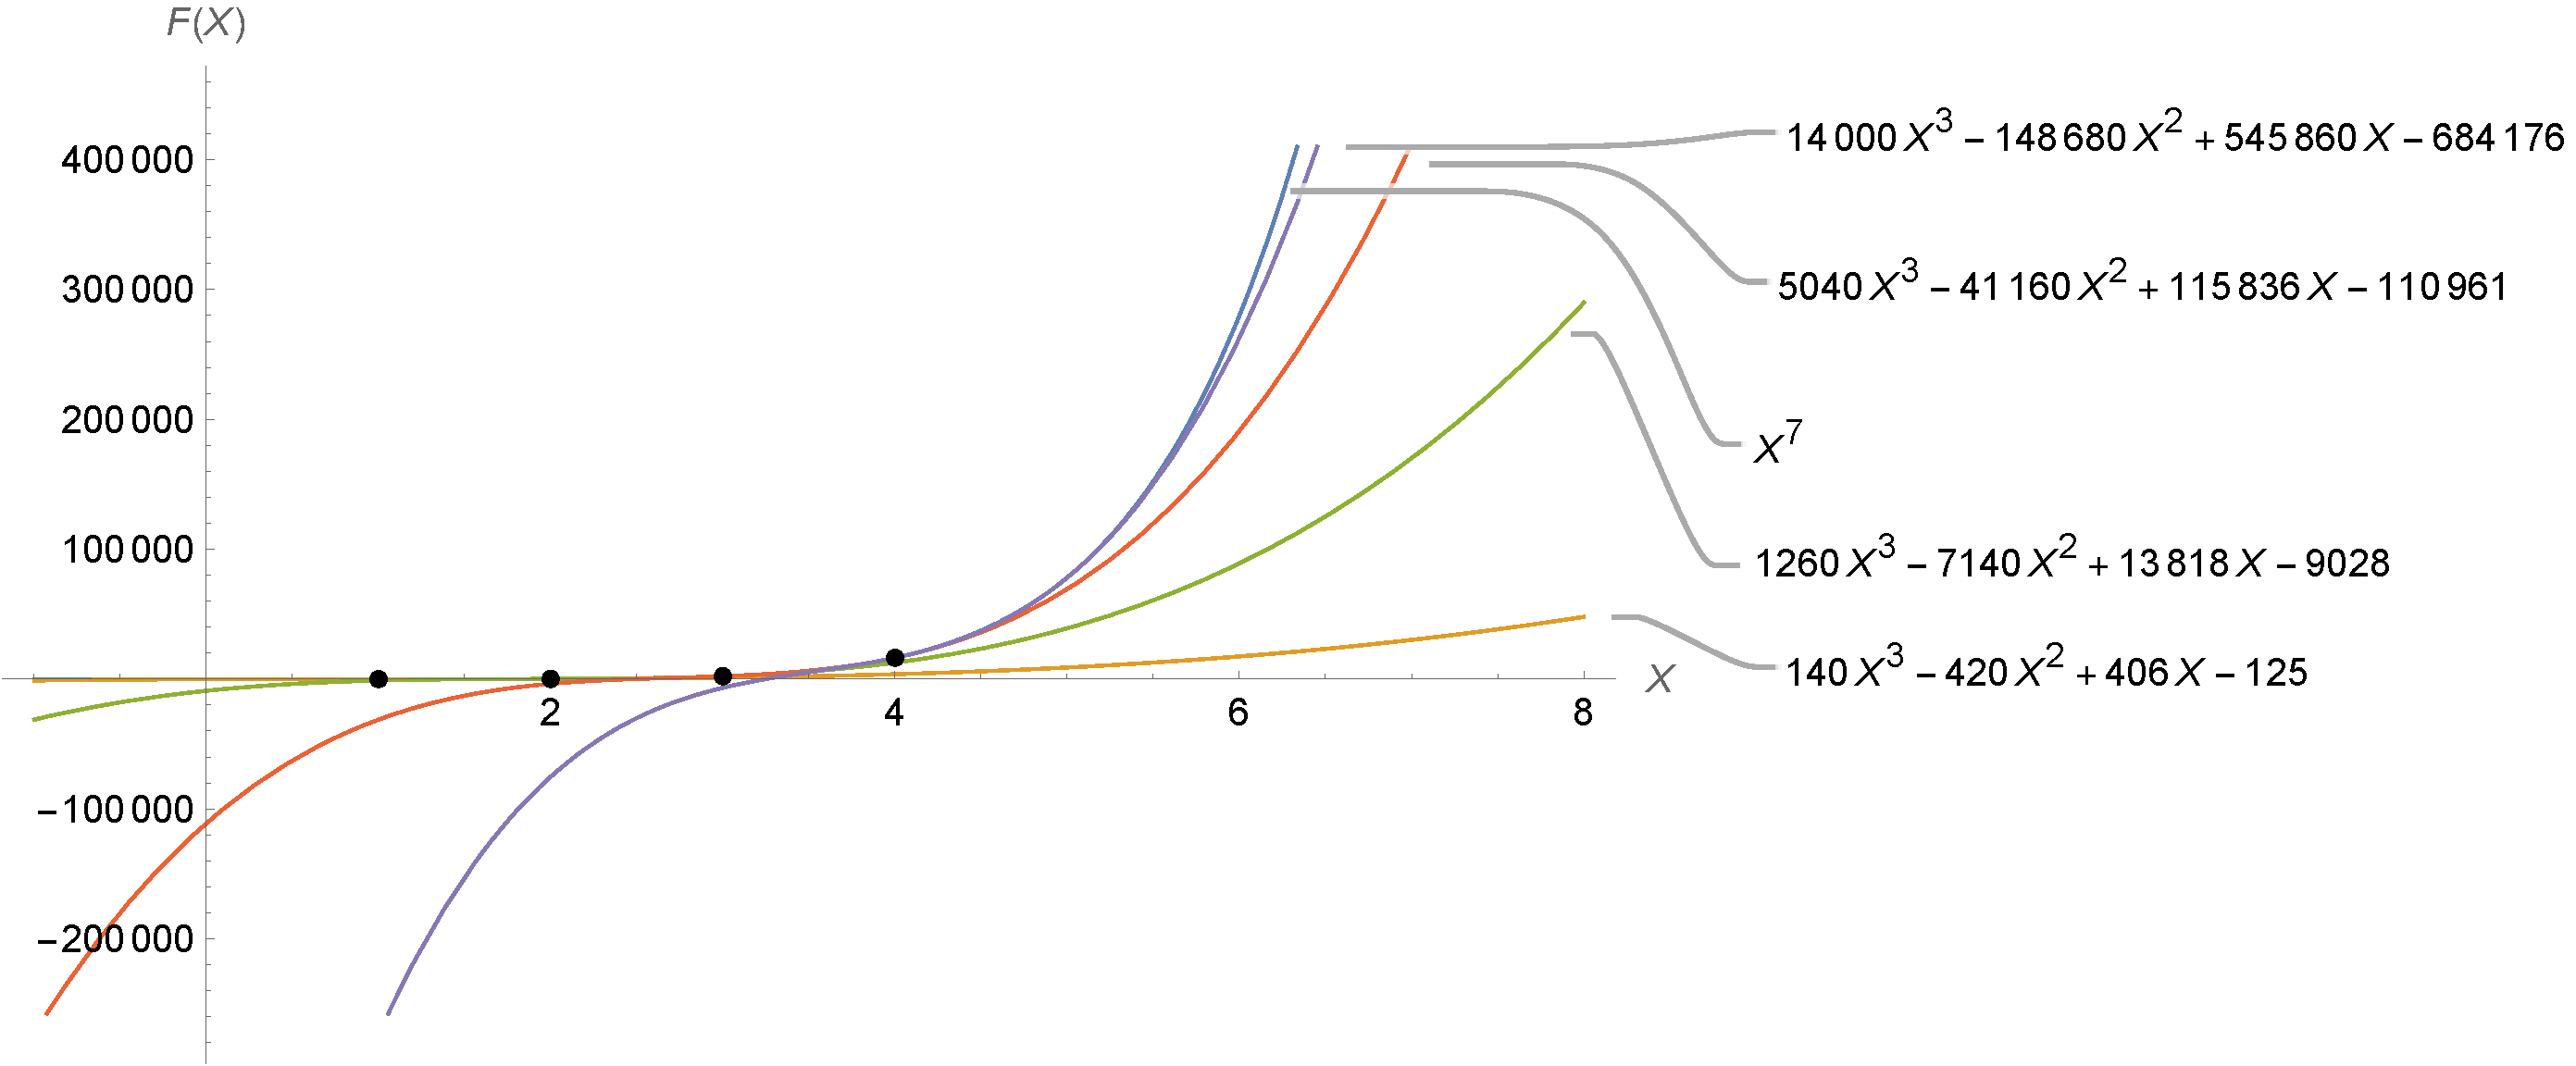
\includegraphics[width=1\textwidth]{sections/images/05_plots_seventh_with_p_3}
    ~\caption{Polynomials P(3, n, k)}\label{fig:figure5}
\end{figure}


    \subsection{Polynomial P(3,X,N) Table of values for N = 3}
    \begin{table}[h!]
    \centering
    \caption{Comparison of $X^7$, $\polynomialP{3}{X}{3} = 5040X^3 - 41160X^2 + 115836X - 110961$, Absolute, Relative, and Percentage Error}
    \begin{tabular}{|c|c|c|c|c|c|}
        \hline
        \textbf{X} & \textbf{$X^7$} & \textbf{$5040X^3 - 41160X^2 + 115836X - 110961$} & \textbf{ABS} & \textbf{Relative} & \textbf{\% Error} \\ \hline
        2.7        & 1046.04        & 942.12                                           & 103.915      & 0.0993421         & 9.93421           \\ \hline
        2.8        & 1349.29        & 1323.48                                          & 25.8129      & 0.0191307         & 1.91307           \\ \hline
        2.9        & 1724.99        & 1728.36                                          & 3.37237      & 0.00195501        & 0.195501          \\ \hline
        3.0        & 2187.00        & 2187.00                                          & 0.0          & 0.0               & 0.0               \\ \hline
        3.1        & 2751.26        & 2729.64                                          & 21.6214      & 0.00785873        & 0.785873          \\ \hline
        3.2        & 3435.97        & 3386.52                                          & 49.4538      & 0.014393          & 1.4393            \\ \hline
        3.3        & 4261.84        & 4187.88                                          & 73.9643      & 0.017355          & 1.7355            \\ \hline
        3.4        & 5252.34        & 5163.96                                          & 88.375       & 0.0168259         & 1.68259           \\ \hline
        3.5        & 6433.93        & 6345.00                                          & 88.9297      & 0.013822          & 1.3822            \\ \hline
        3.6        & 7836.42        & 7761.24                                          & 75.1764      & 0.00959321        & 0.959321          \\ \hline
        3.7        & 9493.19        & 9442.92                                          & 50.2677      & 0.00529514        & 0.529514          \\ \hline
        3.8        & 11441.6        & 11420.3                                          & 21.2783      & 0.00185973        & 0.185973          \\ \hline
        3.9        & 13723.1        & 13723.6                                          & 0.459332     & 0.0000334715      & 0.00334715        \\ \hline
        4.0        & 16384.0        & 16383.0                                          & 1.0          & 0.0000610352      & 0.00610352        \\ \hline
        4.1        & 19475.4        & 19428.8                                          & 46.5874      & 0.00239211        & 0.239211          \\ \hline
        4.2        & 23053.9        & 22891.3                                          & 162.613      & 0.0070536         & 0.70536           \\ \hline
        4.3        & 27181.9        & 26800.7                                          & 381.181      & 0.0140234         & 1.40234           \\ \hline
        4.4        & 31927.8        & 31187.2                                          & 740.621      & 0.0231968         & 2.31968           \\ \hline
        4.5        & 37366.9        & 36081.0                                          & 1285.95      & 0.034414          & 3.4414            \\ \hline
        4.6        & 43581.8        & 41512.4                                          & 2069.33      & 0.0474815         & 4.74815           \\ \hline
        4.7        & 50662.3        & 47511.7                                          & 3150.59      & 0.0621881         & 6.21881           \\ \hline
        4.8        & 58706.8        & 54109.1                                          & 4597.75      & 0.0783172         & 7.83172           \\ \hline
        4.9        & 67822.3        & 61334.8                                          & 6487.55      & 0.0956551         & 9.56551           \\ \hline
        5.0        & 78125.0        & 69219.0                                          & 8906.0       & 0.113997          & 11.3997           \\ \hline
        5.1        & 89741.1        & 77792.0                                          & 11949.0      & 0.13315           & 13.315            \\ \hline
    \end{tabular}\label{tab:table3}
\end{table}


    \subsection{Polynomial P(3,X,3) plot with seventh}
    \begin{figure}[H]
    \centering
    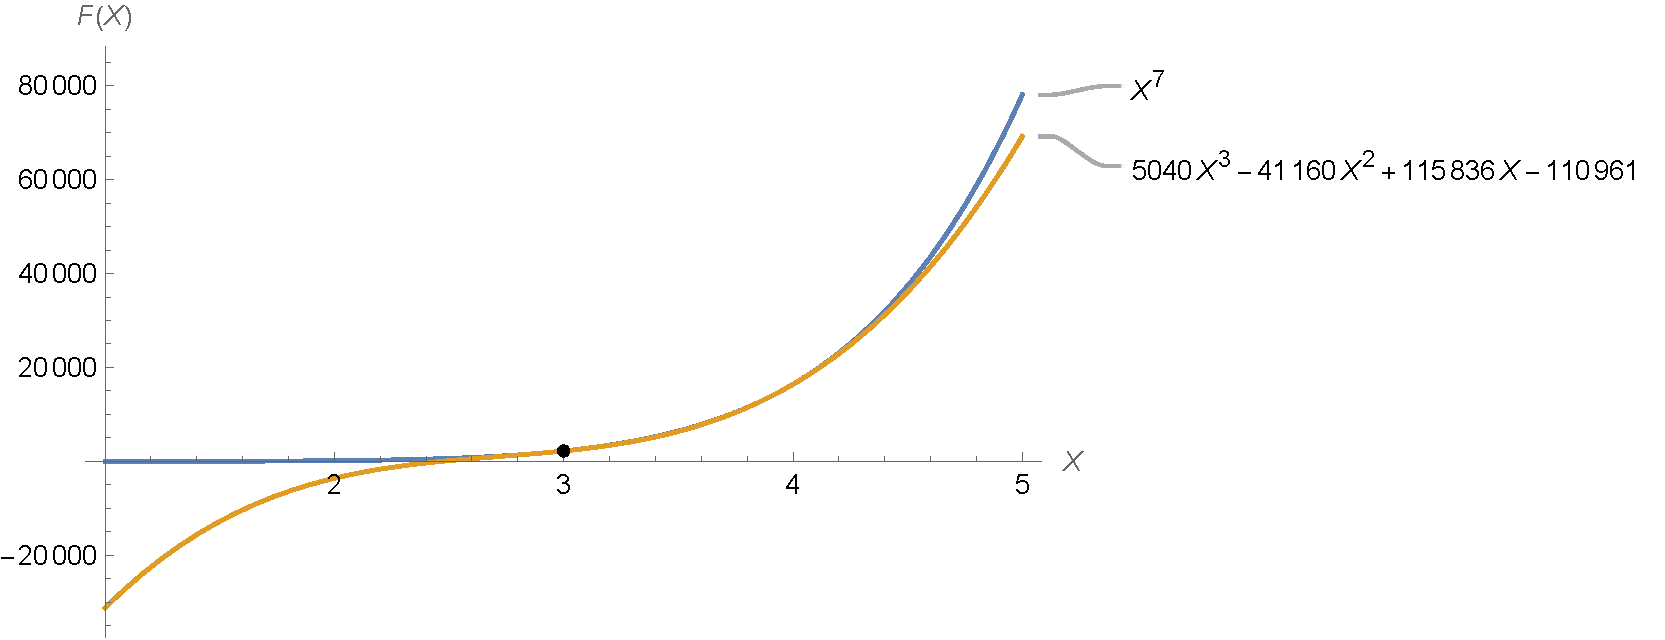
\includegraphics[width=1\textwidth]{sections/images/05_plots_polynomial_p3_n3_with_seventh}
    ~\caption{Polynomial plot P(3, X, 3) with fifth.
    Points of intersection $X=2.87643$, $X=3$, $X=3.89662$, $X=3.99457$.}\label{fig:figure11}
\end{figure}


    % Q3

    \subsection{Polynomials Q(3,X,N)}
    \begin{align*}
    \polynomialQ{3}{X}{0} &= 0 \\
    \polynomialQ{3}{X}{1} &= 1 \\
    \polynomialQ{3}{X}{2} &= 140X^3 - 420X^2 + 406X - 124 \\
    \polynomialQ{3}{X}{3} &= 1260X^3 - 7140X^2 + 13818X - 9027 \\
    \polynomialQ{3}{X}{4} &= 5040X^3 - 41160X^2 + 115836X - 110960 \\
    \polynomialQ{3}{X}{5} &= 14000X^3 - 148680X^2 + 545860X - 684175 \\
    \polynomialQ{3}{X}{6} &= 31500X^3 - 411180X^2 + 1858290X - 2871324 \\
    \polynomialQ{3}{X}{7} &= 61740X^3 - 955500X^2 + 5124126X - 9402659 \\
    \polynomialQ{3}{X}{8} &= 109760X^3 - 1963920X^2 + 12182968X - 25872832 \\
    \polynomialQ{3}{X}{9} &= 181440X^3 - 3684240X^2 + 25945416X - 62572095 \\
    \polynomialQ{3}{X}{10} &= 283500X^3 - 6439860X^2 + 50745870X - 136972700 \\
    \polynomialQ{3}{X}{11} &= 423500X^3 - 10639860X^2 + 92745730X - 276971299 \\
    \polynomialQ{3}{X}{12} &= 609840X^3 - 16789080X^2 + 160386996X - 524988144 \\
    \polynomialQ{3}{X}{13} &= 851760X^3 - 25498200X^2 + 264896268X - 943023887 \\
    \polynomialQ{3}{X}{14} &= 1159340X^3 - 37493820X^2 + 420839146X - 1618774780 \\
    \polynomialQ{3}{X}{15} &= 1543500X^3 - 53628540X^2 + 646725030X - 2672907075 \\
    \polynomialQ{3}{X}{16} &= 2016000X^3 - 74891040X^2 + 965662320X - 4267591424 \\
    \polynomialQ{3}{X}{17} &= 2589440X^3 - 102416160X^2 + 1406064016X - 6616398079 \\
    \polynomialQ{3}{X}{18} &= 3277260X^3 - 137494980X^2 + 2002403718X - 9995653692 \\
    \polynomialQ{3}{X}{19} &= 4093740X^3 - 181584900X^2 + 2796022026X - 14757360515 \\
    \polynomialQ{3}{X}{20} &= 5054000X^3 - 236319720X^2 + 3835983340X - 21343778800
\end{align*}
\begin{figure}[H]
    \centering
    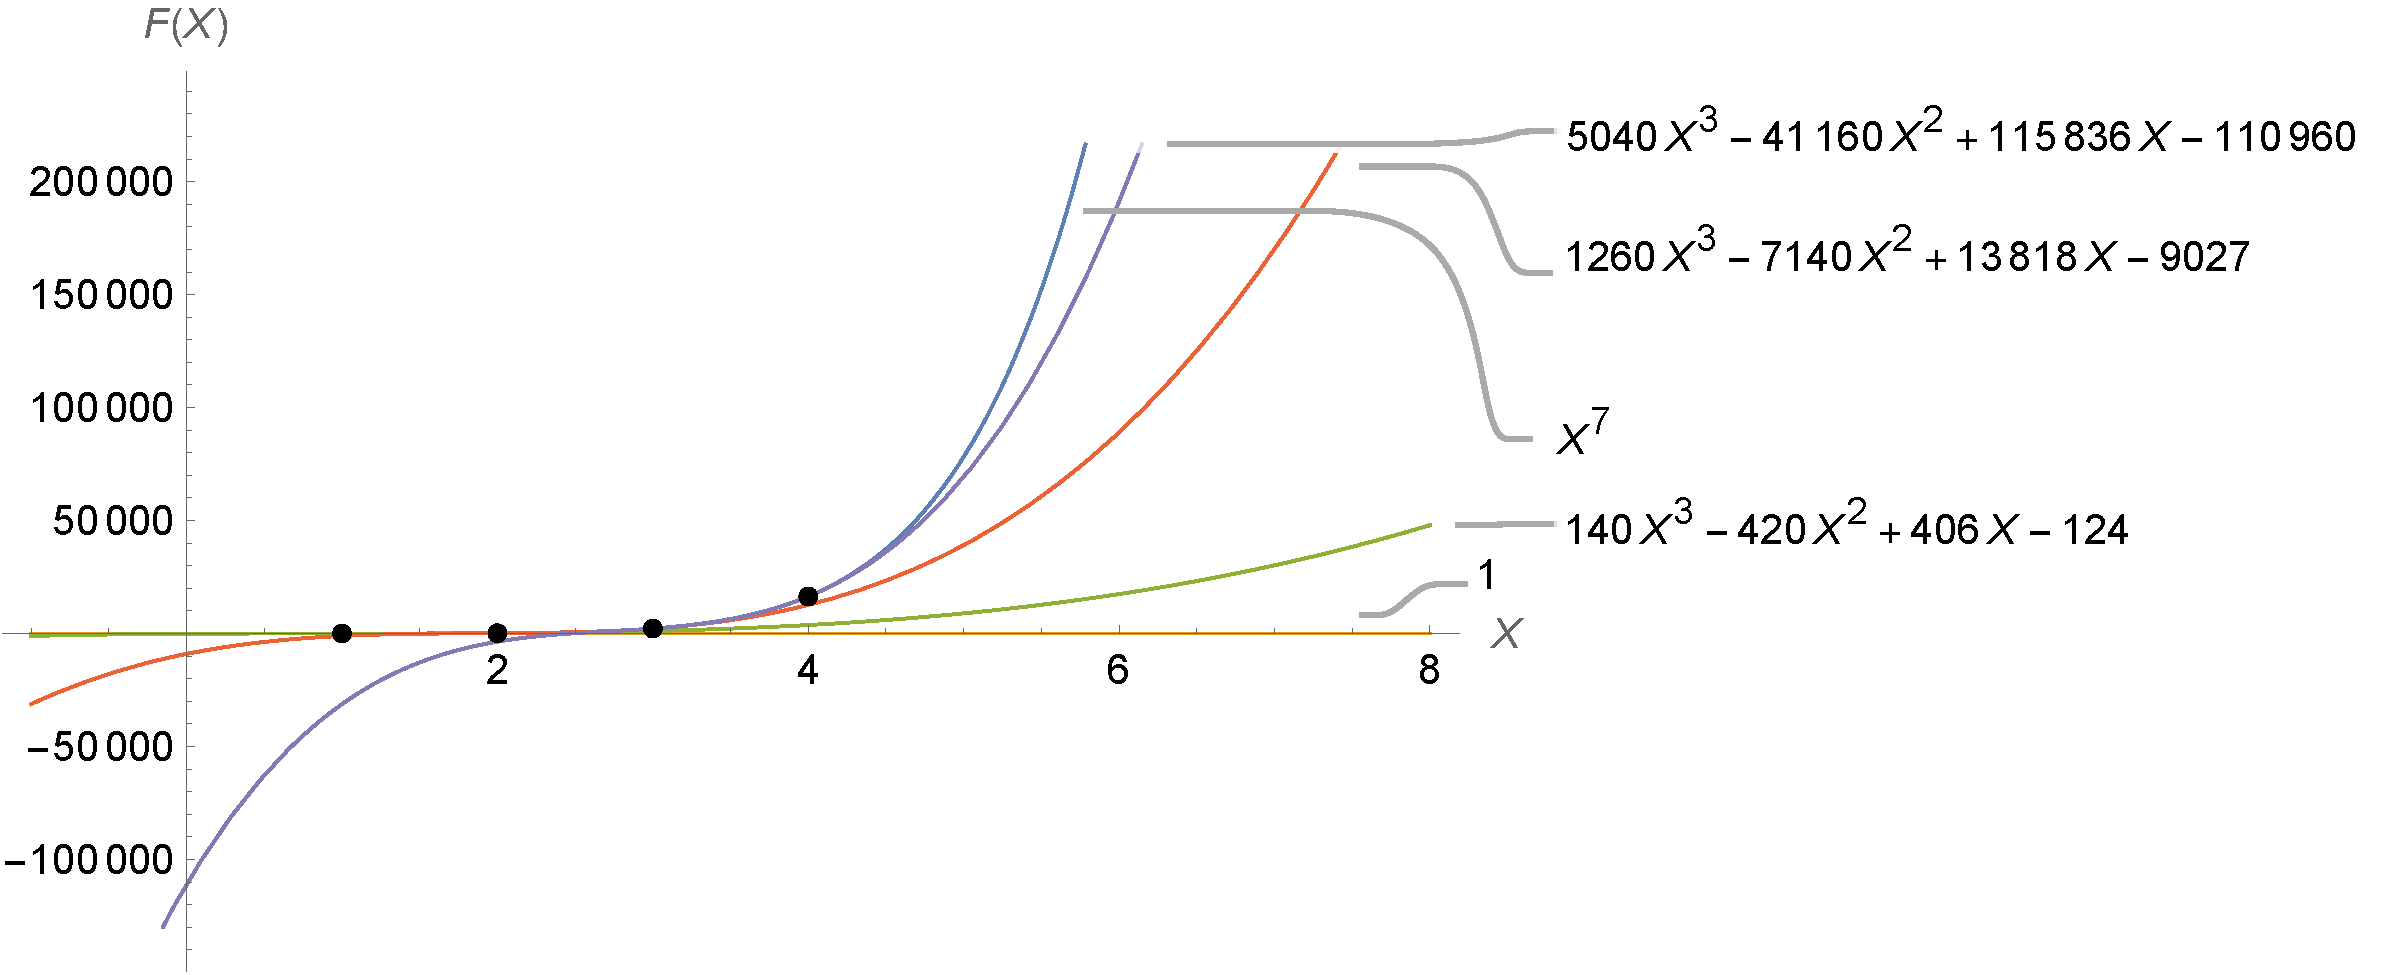
\includegraphics[width=1\textwidth]{sections/images/06_plots_seventh_with_q_3}
    ~\caption{Polynomials Q(3, n, k)}\label{fig:figure6}
\end{figure}


    \subsection{Polynomial Q(3,X,N) Table of values for N = 3}
    \begin{table}[h!]
    \centering
    \caption{Comparison of $X^7$, $\polynomialQ{3}{X}{3} = 1260X^3 - 7140X^2 + 13818X - 9027$, Absolute, Relative, and Percentage Error}
    \begin{tabular}{|c|c|c|c|c|c|}
        \hline
        \textbf{X} & \textbf{$X^7$} & \textbf{$1260X^3 - 7140X^2 + 13818X - 9027$} & \textbf{ABS} & \textbf{Relative} & \textbf{\% Error} \\ \hline
        1.7        & 41.0339        & 19.38                                        & 21.6539      & 0.527707          & 52.7707           \\ \hline
        1.8        & 61.222         & 60.12                                        & 1.102        & 0.0180001         & 1.80001           \\ \hline
        1.9        & 89.3872        & 94.14                                        & 4.75283      & 0.0531712         & 5.31712           \\ \hline
        2.0        & 128.0          & 129.0                                        & 1.0          & 0.0078125         & 0.78125           \\ \hline
        2.1        & 180.109        & 172.26                                       & 7.84885      & 0.0435784         & 4.35784           \\ \hline
        2.2        & 249.436        & 231.48                                       & 17.9558      & 0.0719856         & 7.19856           \\ \hline
        2.3        & 340.483        & 314.22                                       & 26.2625      & 0.0771333         & 7.71333           \\ \hline
        2.4        & 458.647        & 428.04                                       & 30.6071      & 0.0667335         & 6.67335           \\ \hline
        2.5        & 610.352        & 580.5                                        & 29.8516      & 0.0489088         & 4.89088           \\ \hline
        2.6        & 803.181        & 779.16                                       & 24.021       & 0.0299074         & 2.99074           \\ \hline
        2.7        & 1046.04        & 1031.58                                      & 14.4553      & 0.0138192         & 1.38192           \\ \hline
        2.8        & 1349.29        & 1345.32                                      & 3.97285      & 0.0029444         & 0.29444           \\ \hline
        2.9        & 1724.99        & 1727.94                                      & 2.95237      & 0.00171153        & 0.171153          \\ \hline
        3.0        & 2187.0         & 2187.0                                       & 0.0          & 0.0               & 0.0               \\ \hline
        3.1        & 2751.26        & 2730.06                                      & 21.2014      & 0.00770607        & 0.770607          \\ \hline
        3.2        & 3435.97        & 3364.68                                      & 71.2938      & 0.0207492         & 2.07492           \\ \hline
        3.3        & 4261.84        & 4098.42                                      & 163.424      & 0.0383459         & 3.83459           \\ \hline
        3.4        & 5252.34        & 4938.84                                      & 313.495      & 0.0596868         & 5.96868           \\ \hline
        3.5        & 6433.93        & 5893.5                                       & 540.43       & 0.0839968         & 8.39968           \\ \hline
        3.6        & 7836.42        & 6969.96                                      & 866.456      & 0.110568          & 11.0568           \\ \hline
        3.7        & 9493.19        & 8175.78                                      & 1317.41      & 0.138774          & 13.8774           \\ \hline
    \end{tabular}\label{tab:table6}
\end{table}


    \subsection{Polynomial Q(3,X,3) plot with seventh}
    \begin{figure}[H]
    \centering
    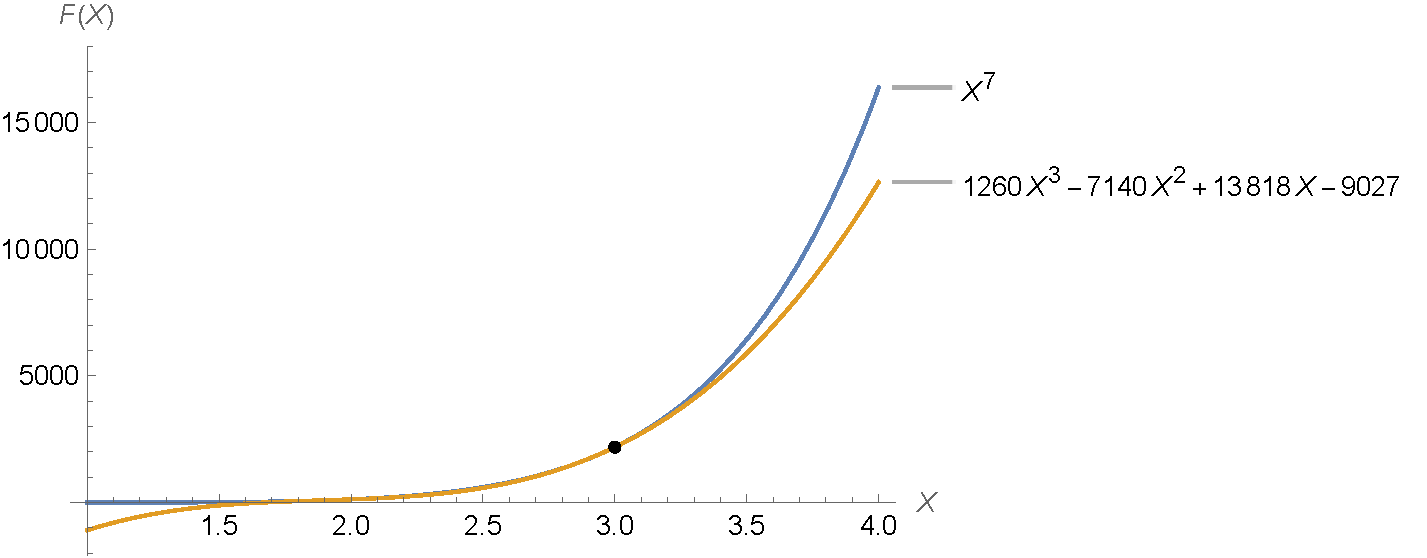
\includegraphics[width=1\textwidth]{sections/images/06_plots_polynomial_q3_n3_with_seventh}
    ~\caption{Polynomial plot $Q(3, X, 3)$ with seventh power $X^7$.
    Points of intersection $X=1.80948$, $X=2.01364$, $X=2.84612$, $X=3$.
    Interval of convergence: $a \leq X \leq b$.
    }\label{fig:figure12}
\end{figure}


\end{document}
